\documentclass[UTF8,12pt]{article} % 12pt 为字号大小
\usepackage{amssymb,amsfonts,amsthm}
%\usepackage{fontspec,xltxtra,xunicode}
%\usepackage{times}
\usepackage{amsmath,bm}
\usepackage{mdwlist}
\usepackage[colorlinks,linkcolor=blue]{hyperref}
\usepackage{cleveref}

%----------
% 定义中文环境
%----------

\usepackage{xeCJK}
\usepackage{float}
\setCJKmainfont[BoldFont={Heiti SC Light},ItalicFont={Kaiti SC Regular}]{Songti SC Regular}
\setCJKsansfont{Heiti SC Light}
\setCJKfamilyfont{song}{Songti SC Regular}
\setCJKfamilyfont{zhhei}{Heiti SC Light}
\setCJKfamilyfont{zhkai}{Kaiti SC Regular}
\setCJKfamilyfont{zhfs}{STFangsong}
\setCJKfamilyfont{zhli}{Libian SC Regular}
\setCJKfamilyfont{zhyou}{Yuanti SC Regular}

\newcommand*{\songti}{\CJKfamily{zhsong}} % 宋体
\newcommand*{\heiti}{\CJKfamily{zhhei}}   % 黑体
\newcommand*{\kaiti}{\CJKfamily{zhkai}}  % 楷体
\newcommand*{\fangsong}{\CJKfamily{zhfs}} % 仿宋
\newcommand*{\lishu}{\CJKfamily{zhli}}    % 隶书
\newcommand*{\yuanti}{\CJKfamily{zhyou}} % 圆体

%----------
% 版面设置
%----------
%首段缩进
\usepackage{indentfirst}
\setlength{\parindent}{2em}

%行距
\renewcommand{\baselinestretch}{1.2} % 1.2倍行距

%页边距
\usepackage[a4paper]{geometry}
\geometry{verbose,
  tmargin=2cm,% 上边距
  bmargin=2cm,% 下边距
  lmargin=2.5cm,% 左边距
  rmargin=2.5cm % 右边距
}


%----------
% 其他宏包
%----------
%图形相关
\usepackage[x11names]{xcolor} % must before tikz, x11names defines RoyalBlue3
\usepackage{graphicx}
\graphicspath{{figures/}}
\usepackage{pstricks,pst-plot,pst-eps}
\usepackage{subfig}
\def\pgfsysdriver{pgfsys-dvipdfmx.def} % put before tikz
\usepackage{tikz}

%原文照排
\usepackage{verbatim}

%网址
\usepackage{url}

%----------
% 定理、习题与解答环境
%----------
%定理环境
\usepackage[most]{tcolorbox}
\newtcbtheorem[number within=section]{theorem}{Theorem}{
     enhanced,
     breakable,
     sharp corners,
     attach boxed title to top left={
       yshifttext=-1mm
     },
     colback=white,
     colframe=blue!75!black,
     fonttitle=\bfseries,
     boxed title style={
       sharp corners,
       size=small,
       colback=blue!75!black,
       colframe=blue!75!black,
     } 
}{theorem}

\newtcbtheorem[number within=section]{definition}{Definition}{
     enhanced,
     breakable,
     sharp corners,
     attach boxed title to top left={
       yshifttext=-1mm
     },
     colback=white,
     colframe=blue!75!black,
     fonttitle=\bfseries,
     boxed title style={
       sharp corners,
       size=small,
       colback=blue!75!black,
       colframe=blue!75!black,
     } 
}{definition}

\newtcbtheorem[number within=section]{corollary}{Corollary}{
     enhanced,
     breakable,
     sharp corners,
     attach boxed title to top left={
       yshifttext=-1mm
     },
     colback=white,
     colframe=blue!75!black,
     fonttitle=\bfseries,
     boxed title style={
       sharp corners,
       size=small,
       colback=blue!75!black,
       colframe=blue!75!black,
     } 
}{Corollary}

%习题环境
\newtcbtheorem[]{exercise}{Problem}{
     enhanced,
     breakable,
     sharp corners,
     attach boxed title to top left={
       yshifttext=-1mm
     },
     colback=white,
     colframe=black,
     fonttitle=\bfseries,
     boxed title style={
       sharp corners,
       size=small,
       colback=black,
       colframe=black,
     } 
}{Problem}

%解答环境
\ifx\proof\undefined\
\newenvironment{proof}[1][\protect\proofname]{\par
\normalfont\topsep6\p@\@plus6\p@\relax
\trivlist
\itemindent\parindent
\item[\hskip\labelsep
\scshape
#1]\ignorespaces
}{%
\endtrivlist\@endpefalse
}
\fi

\renewcommand{\proofname}{\it{Solution}}

%----------
%示例:
%\begin{exs} \end{exs}
%\begin{proof}[] \end{proof}
%\begin{thm}{}{} \end{thm}
%----------

%----------
%插入图片
%\begin{figure}[htbp]
%\centering
%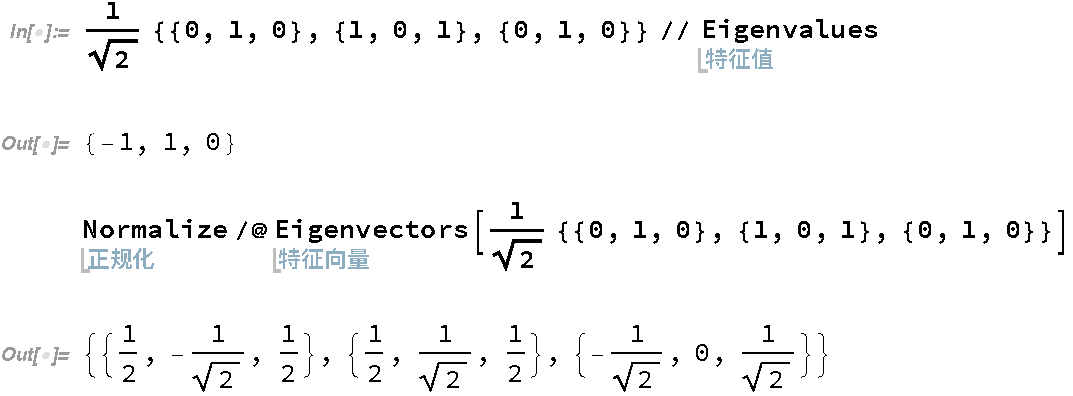
\includegraphics[width=10cm]{eigen}
%\end{figure}
%----------

%==========
% 正文部分
%==========

\begin{document}

\title{Homework 01}
\author{陈昱全~SA18234049}
\date{} % 若不需要自动插入日期,则去掉前面的注释;{ } 中也可以自定义日期格式
\maketitle

\begin{exercise}{1.1}{}
Prove $$[AB,CD] = -AC\{D,B\} + A\{C,B\}D - C\{D,A\}B + \{C,A\}DB$$
\end{exercise}

\begin{proof}[Proof]
\begin{align*}
&[AB,CD] = ABCD - CDAB \\
&= ABCD - CDAB + (CADB - CADB) + (ACDB - ACDB) + (ACBD - ACBD) \\
&= (- ACDB - ACBD) + (ACBD + ABCD) - (CDAB - CADB) + (CADB + ACDB) \\
&= -AC\{D,B\} + A\{C,B\}D - C\{D,A\}B + \{C,A\}DB
\end{align*}
\end{proof}

\begin{exercise}{1.4}{}
Using the rules of bra-ket algebra, prove or evaluate the following:\\
\textbf{(a)} $tr(XY) = tr(YX)$, where $X$ and $Y$ are operators.\\
\textbf{(b)} $(XY)^\dagger = Y^\dagger X^\dagger$, where $X$ and $Y$ are operators.\\
\textbf{(c)} $exp[if(A)] = ?$ in ket-bra form, where $A$ is a Hermitian operator whose eigenvalues are known.\\
\textbf{(d)} $\sum_{a'}\psi_{a'}^{*}(\bm{x'})\psi_{a'}(\bm{x''})$, where $\psi_{a'}(\bm{x'}) = \langle\bm{x'}|a'\rangle$.
\end{exercise}

\begin{proof}
Suppose we have a normalized orthogonal basis $\{|\alpha_i\rangle\} = \{|\alpha_1\rangle, ... , |\alpha_n\rangle\}$, all the operators in this problem will be represented under $\{|\alpha_i\rangle\}$.\\
\textbf{(a)} The $i$th element on the diagonal of the matrix $XY$ is:
$$(XY)_i = X_{i1}Y_{1i} + X_{i2}Y_{2i} + ... + X_{in}Y_{ni} = \sum_{j=1}^{n} X_{ij}Y_{ji}$$
then
$$tr(XY) = \sum_{i=1}^{n}\sum_{j=1}^{n} X_{ij}Y_{ji} = \sum_{j=1}^{n}\sum_{i=1}^{n} Y_{ji}X_{ij} = tr(YX)$$
\textbf{(b)} By definition, for any state $|\alpha \rangle$, we define $X^\dagger$ as:
$$(X|\alpha \rangle)^\dagger = \langle \alpha|X^\dagger$$
so
$$(XY|\alpha \rangle)^\dagger = (Y|\alpha \rangle)^\dagger X^\dagger = \langle \alpha|Y^\dagger X^\dagger$$
which means
$$(XY)^\dagger = Y^\dagger X^\dagger$$
\textbf{(c)} By another definition of function of operators (see \textit{Quantum Computation and Quantum Information, Michael A. Nielsen, Anniversary edition} page 75), we first write
$$A = \sum_{i} a_i |i\rangle\langle i|$$
where $|i\rangle$ is the eigenvector of $A$, and $a_i$ is the corresponding eigenvalue. Then by definition,
$$e^{if(A)} = \sum_{i} e^{ia_i} |i\rangle\langle i|$$
\textbf{(d)} We have $\psi_{a'}(\bm{x'}) = \langle\bm{x'}|a'\rangle$, $\psi_{a'}^*(\bm{x'}) = \langle a'|\bm{x'}\rangle$, $\psi_{a'}(\bm{x''}) = \langle\bm{x''}|a'\rangle$, so
\begin{align*}
\sum_{a'}\psi_{a'}^{*}(\bm{x'})\psi_{a'}(\bm{x''}) &= \sum_{a'} \langle a'|\bm{x'}\rangle \langle\bm{x''}|a'\rangle \\
&= \sum_{a'} \langle\bm{x''}|a'\rangle \langle a'|\bm{x'}\rangle \\
&= \langle\bm{x''}|\left(\sum_{a'} |a'\rangle \langle a'|\right) |\bm{x'}\rangle \\
&= \langle\bm{x''}|\bm{x'}\rangle
\end{align*}
\end{proof}

\begin{exercise}{1.6}{}
Suppose $|i\rangle$ and $|j\rangle$ are eigenkets of some Hermitian operator $A$. Under what condition can we conclude that $|i\rangle + |j\rangle$ is also an eigenket of $A$? Justify your answer.
\end{exercise}

\begin{proof}
The condition is: $|i\rangle$ and $|j\rangle$ corresponding to the same eigenvalue.

Suppose $|i\rangle$ and $|j\rangle$ corresponding to the same eigenvalue $\alpha$, we have
$$A|i\rangle = \alpha |i\rangle,~A|j\rangle = \alpha |j\rangle$$
so
$$A(|i\rangle + |j\rangle) = \alpha |i\rangle + \alpha |j\rangle = \alpha (|i\rangle + |j\rangle),$$
then $(|i\rangle + |j\rangle)$ is also an eigenket of $A$.
\end{proof}

\begin{exercise}{1.14}{}
A certain observable in quantum mechanics has a $3\times 3$ matrix representation as follows:
$$\frac{1}{\sqrt{2}} \begin{pmatrix} 0 & 1 & 0 \\ 1 & 0 & 1 \\ 0 & 1 & 0 \end{pmatrix}$$
\textbf{(a)} Find the normalized eigenvectors of this observable and the corresponding eigenvalues. Is there any degeneracy?\\
\textbf{(b)} Give a physical example where all this is relevant.
\end{exercise}

\begin{proof}
Let the observable in the problem as $A$.\\
\textbf{(a)} Let  $\lambda$ as the eigenvalue, we have $A|\alpha \rangle = \lambda |\alpha \rangle \Rightarrow (A - \lambda I)|\alpha \rangle = 0$. So there is
$$det(A - \lambda I) = 0$$
we can get the solution $\lambda = -1, 1, 0$ and the corresponding eigenkets
$$|\alpha_1\rangle = \frac{1}{2}\begin{pmatrix} 1 \\ -\sqrt{2} \\ 1 \end{pmatrix},~ |\alpha_2\rangle = \frac{1}{2}\begin{pmatrix} 1 \\ \sqrt{2} \\ 1 \end{pmatrix},~ |\alpha_1\rangle = \frac{1}{\sqrt{2}}\begin{pmatrix} -1 \\ 0 \\ 1 \end{pmatrix}$$
So there's no degeneracy.
Here, we can also use \textit{Mathematica} to get the eigenkets and the corresponding eigenvalues.
\begin{figure}[htbp]
\centering
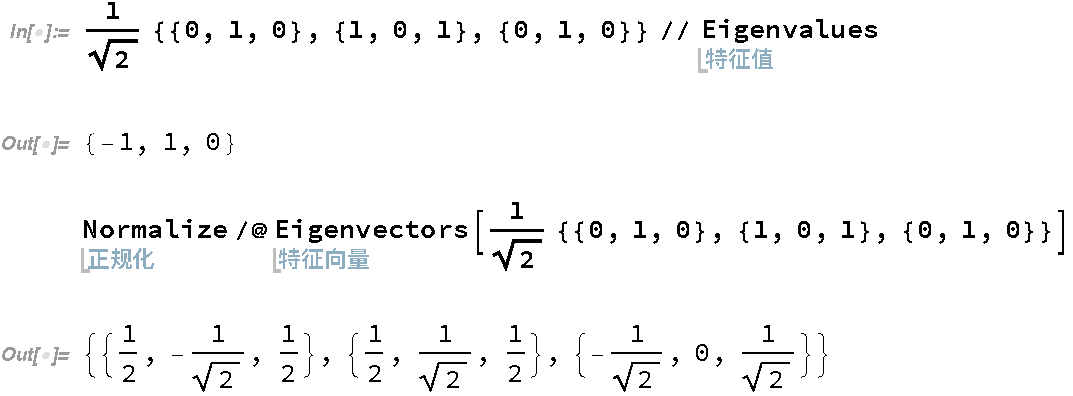
\includegraphics[width=10cm]{eigen}
\end{figure}\\
\textbf{(b)} Due to $A$ is Hermitian, we can regard $A$ as a Hamiltonian, so the different eigenvalues of $A$ represent different energy level of $A$, and these corresponding eigenvectors are the eigenstates. 
\end{proof}

\begin{exercise}{Additional}{}
If operator $U$ satisfies $UU^\dagger = I$ in a certain representation, show this is true for any other representations.
\end{exercise}

\begin{proof}[Proof]
Suppose we have an orthogonal normalized basis $\{|\alpha_i\rangle\}$ and an operator $\hat{U}$, let $U$ to be the corresponding matrix representation under basis $\{|\alpha_i\rangle\}$. So we have
$$U_{ij} = \langle\alpha_i|\hat{U}|\alpha_j\rangle$$\\
Let $\{|\alpha'_i\rangle\}$ be a new orthogonal normalized basis, so the new basis could be represented under the old basis $\{|\alpha_i\rangle\}$:
$$|\alpha'_i\rangle = \sum_j S_{ji}|\alpha_j\rangle$$
or we can simply write it as:
$$|\alpha'_i\rangle = S|\alpha_i\rangle$$
where $S$ is a unitary operator under basis $\{|\alpha_i\rangle\}$.\\
Let $U'$ to be the corresponding matrix representation of $\hat{U}$ under new basis $\{|\alpha'_i\rangle\}$, we have
$$U' = S^{-1}US = S^\dagger US$$
then
\begin{align*}
U'U'^\dagger &= S^\dagger US(S^\dagger US)^\dagger \\
&= S^\dagger US\cdot (US)^\dagger S \\
&= S^\dagger US\cdot S^\dagger U^\dagger S \\
&= S^\dagger UU^\dagger S = S^\dagger S = I
\end{align*}
\end{proof}

\end{document}